\documentclass[12pt,a4paper]{book}

\usepackage[portuguese]{babel}

\usepackage{graphicx}
\usepackage[colorlinks=true, allcolors=black]{hyperref}

\usepackage{enumitem}
\setitemize{fullwidth}
\setenumerate{wide}

\usepackage{longtable}
\renewcommand{\arraystretch}{1.5}

\usepackage{indentfirst}

\usepackage[nottoc,numbib]{tocbibind}
\addto\captionsportuguese{
  \renewcommand{\bibname}{Referências}
  \renewcommand{\contentsname}{Índice}
}
\usepackage{shorttoc}
\addtocontents{toc}{\protect\thispagestyle{empty}}
\pagenumbering{gobble}

\title{Como Jogar Go: Uma Introdução Concisa}
\author{Richard Bozulich e James Davies\\[1ex] 
\small{traduzido por Philippe Fanaro}}
\date{}

\begin{document}
    \maketitle
    \shorttoc{Índice Resumido}{0}
    \tableofcontents

    \frontmatter
    \chapter{Prefácio}

Go é o jogo de tabuleiro oriental milenar jogado por milhões de pessoas ao redor do mundo. As regras são tão fáceis que uma criança de cinco anos pode aprendê-lo, porém, a verdadeira maestria demanda anos de estudos intensivos. Como a natureza, seus simples elementos --- madeira e pedra, linha e círculo, preto e branco --- constroem estruturas complexas.

Go é o jogo perfeito para se desenvolver habilidades tanto do lado esquerdo quanto direito do cérebro --- intuição e reconhecimento de padrões, assim como análise por força bruta. Adicionalmente, a riqueza de seus conceitos estratégicos permitem que o Go seja utilizado como modelo para tomadas de decisões na vida real.

Go também ensina o valor da paciência, além de demonstrar como balancear agressividade e prudência para ganhos máximos.

\bigskip

\emph{Como Jogar Go: Uma Introdução Concisa}~\cite{bozulich_how_to_play_go} é uma introdução simples e direta ao jogo. As 10 regras básicas são claramente explicadas em somente algumas páginas. Problemas são intercalados durante o livro, para ajudar na compreensão dos conceitos sendo apresentados. Após as regras terem sido detalhadamente exploradas, há uma seção sobre estratégias de abertura, seguida de uma outra sobre táticas. Tudo que é essencial à prática do jogo está incluído com diversas referências a recursos que ajudarão o leitor a continuar em sua jornada neste milenar e profundo jogo.

\bigskip
\bigskip

Richard Bozulich

20 de Dezembro de 2016
    \chapter{Nota do Tradutor}

Primeiramente, agradeço muito ao Richard Bozulich e ao James Davies por, não somente terem escrito este livro mas, também, terem liberados os direitos de tradução. Espero que seja o primeiro de muitos livros da excelente editora Kiseido~\cite{kiseido} traduzidos para o português.

\bigskip

A tradução deste livro foi feita com base em meu conhecimento do jogo. Sou um jogador amador de força aproximada mínima de 1 dan\footnote{Seria supostamente equivalente ao de faixa preta em artes marciais. Mas essa é uma simplificação talvez grosseira e discutível, uma comparação à la banana versus maçã.}, um ranking tido como de maestria do jogo, apesar de que, claro, sempre há um peixe maior. Desde que comecei a jogar no final de 2012, já participei de torneios tanto no Brasil quanto na Europa, na Coreia e na China, além de alguns torneios online também. Toda essa experiência me ajuda a discernir o que é bom do que é ruim, o que é útil do que é perda de tempo.

É por isso que corri atrás de conteúdo da editora Kiseido, que vem trazendo ao Ocidente, em inglês, conhecimento de Go já há décadas. No caso deste livro, temos uma introdução sólida e sistemática ao jogo, com muita concisão. Nele, o leitor encontrará, além das regras, conceitos e técnicas utilizadas por desde iniciantes até grandes mestres do Go, e táticas e estratégias que residem no coração jogo.

Porém, não tenha pressa. Go demanda muita prática, e esta é muito divertida e recompensadora. Internalizar os conceitos deste livro é algo que não só demanda tempo, mas que também é feito em ciclos, mesmo os grandes mestres aprendem com os fundamentos todos os dias.

\pagebreak

Após o término deste livro, infelizmente, não há muito mais conteúdo em português, pelo menos não em livros outras vias impressas. Tentarei continuar criando mais traduções de livro de Go, mas não sei a que velocidade ou até que ponto. No entanto, já há conteúdo online para variados níveis, em português, espalhado pela internet. E também vale ressaltar que, mesmo livros em línguas estrangeiras, muitas vezes são compreensíveis pois diagramas de Go são uma linguagem à parte e universal.

Algumas dessas outras fontes com mais conteúdo são --- há já muitos canais de YouTube e de Twitch em diversas línguas também ---:

\begin{longtable}{l|p{60mm}} 
 \hline
 \textbf{Nome ou URL} & \textbf{Descrição} \\
 \hline \hline
 \href{https://online-go.com}{\path{online-go.com}}~\cite{ogs} & o servidor OGS é essencialmente uma versão mais moderna do servidor KGS, citado no livro. A interface é mais bem feita e há muitos outros recursos, incluindo tutoriais e josekipédia. Este é o servidor que eu mais recomendo para iniciantes \\
 \hline
 \href{https://facebook.com/groups/gobrasil}{\path{facebook.com/groups/gobrasil}}~\cite{facebook_go_brasil} & grupo \emph{Go Brasil} no Facebook, com mais de 1200 integrantes. Também há um grupo de Whatsapp bastante ativo, mas será preciso demandar pelo grupo de Facebook como acessá-lo \\
 \hline
 \href{https://nihonkiin.com.br}{\path{nihonkiin.com.br}}~\cite{brasil_nihon_kiin} & site da Brasil Nihon Kiin, associação nipo-brasileira de Go, que, também, existe fisicamente em São Paulo-SP \\
 \hline
 \href{https://shin.gokgs.com/}{\path{shin.gokgs.com}}~\cite{shinkgs} & uma nova fachada para o servidor KGS, totalmente integrada em navegadores \\
 \hline
 \emph{Go --- Coleção Jogos de Tabuleiro}~\cite{go_sao_paulo} & um livro similar a este, criado pela Secretaria Municipal de São Paulo em conjunto com a Brasil Nihon Kiin, também de São Paulo \\
 \hline
 \href{https://fanaro.io}{\path{fanaro.io}}~\cite{fanaroio} & meu site, com conteúdo não só de Go \\
 \hline
 \href{https://youtube.com/c/PhilippeFanaro}{\path{youtube.com/c/PhilippeFanaro}}~\cite{fanaro_youtube} & meu canal de YouTube, focado em Go \\
 \hline
 \href{https://twitch.tv/fanaro009}{\path{twitch.tv/fanaro009}}~\cite{fanaro_twitch} & meu canal de Twitch, onde jogo e ensino ao vivo, ocasionalmente \\
 \hline
\end{longtable}

\pagebreak

Por fim, gostaria de comentar que muitos dos termos técnicos de Go traduzidos por mim ao longo do livro encontram suas primeiras instâncias em português. Ou seja, não os leve tanto a ferro e fogo, inclusive pois a maioria dos jogadores veteranos na verdade utiliza as respectivas versões japonesas. Tanto o autor original quanto eu, o tradutor, optamos por minimizar a carga de vocabulário para quem está começando.

\bigskip
\bigskip

\emph{Sua jornada só está começando, e um guia completo como este será de grande valia na sua aventura pelo jogo e sua respectiva filosofia.}

\bigskip
\bigskip

Para mais informações, ou caso queira fornecer feedback, melhorias ou comentários, é só enviar um email para \emph{\href{mailto:philippefanaro@gmail.com}{philippefanaro@gmail.com}}~\cite{fanaro_email}. Este livro/projeto também é código-aberto, ou seja, é possível examinar detalhadamente como ele foi feito, através da ferramenta \LaTeX~\cite{latex} pelo link \href{https://github.com/FanaroEngineering/traducao_como_jogar_go}{\path{github.com/.../traducao_como_jogar_go}}~\cite{repo_github}.

\bigskip
\bigskip

Philippe Fanaro

1 de Outubro de 2021
    \chapter{Glossário de Termos de Go Utilizados Neste Livro}

\begin{longtable}{l|p{100mm}} 
 \hline
 \textbf{Termo} & \textbf{Significado} \\
 \hline \hline
 \textbf{atari} & quando todas as intersecções exceto um diretamente adjacente à pedra ou grupo de pedras são ocupadas pelo oponente, a pedra ou grupo é dita estar sob ``atari", e o oponente pode capturá-la no próximo movimento \\ 
 \hline
 \textbf{dan} & uma classificação indo de shodan (1 dan) até 9 dan \\
 \hline
 \textbf{gote} & um movimento que o oponente pode ignorar. Um movimento gote é geralmente defensivo, então não representa nenhuma ameaça ao adversário. \\
 \hline
 \textbf{joseki} & durante a abertura, conflitos locais frequentemente surgem, começando tipicamente nos cantos e se desenvolvendo para os lados. Esses conflitos locais se chamam josekis \\
 \hline
 \textbf{komi} & compensação de pontos adicionada a um dos lados no final da partida. Tipicamente, 6.5 pontos ao território do Branco em uma partida igual, para compensar a desvantagem de ser a segunda cor a jogar. \\
 \hline
 \textbf{kyu} & uma classificação amadora indo desde aproximadamente 35 kyu (um total iniciante) até 1 kyu, o mais alto nível antes de shodan (1 dan) \\
 \hline
 \textbf{nigiri} & um procedimento para escolher quem joga primeiro em uma partida igual. Veja a página 71. \\
 \hline
 \textbf{Nihon Kiin} & a Associação de Go do Japão. Uma fundação sem fins lucrativos baseada em Tóquio com cerca de 300 profissionais ativos. Somente jogadores pertencentes a essa organização ou à Associação Ocidental de Go do Japão são permitidos a competir em torneios japoneses patrocinados por jornais ou empresas \\
 \hline
 \textbf{tesuji} & um movimento habilidoso que conquista um objetivo tático claro \\
 \hline
 \textbf{sanrensei} & um padrão de abertura em que um jogador ocupa três pontos-estrela em um dos lados do tabuleiro \\
 \hline
 \textbf{san-san} & o ponto 3-3 em qualquer um dos cantos \\
 \hline
 \textbf{sente} & um movimento que o oponente não pode ignorar, caso contrário ele sofrerá uma perda inaceitável \\
 \hline
 \textbf{seki} & vida mútua. Uma situação em que nenhum dos dois grupos de cores opostas possui dois olhos, mas nenhum dos lados pode atacar o outro sem perder suas próprias pedras \\
 \hline
\end{longtable}

    \mainmatter
    \chapter{O Equipamento}

Go é geralmente jogado em um tabuleiro com 19 linhas verticais e 19 horizontais, constituindo uma grade de 361 intersecções, como se pode ver pelo \emph{Diagrama 1}. O tabuleiro possui nove pontos grifados com pequenos círculos. Esses círculos são chamados de pontos-estrela.

As peças ou pedras são tipicamente duplo-convexas, para facilitar o manuseio quando de muitas pedras em uma mesma área. Um conjunto de Go padrão possui 181 pedras pretas e 180 pedras brancas.

\begin{wrapfigure}{r}{60mm}
    \vspace{-20pt}
    \begin{center}
        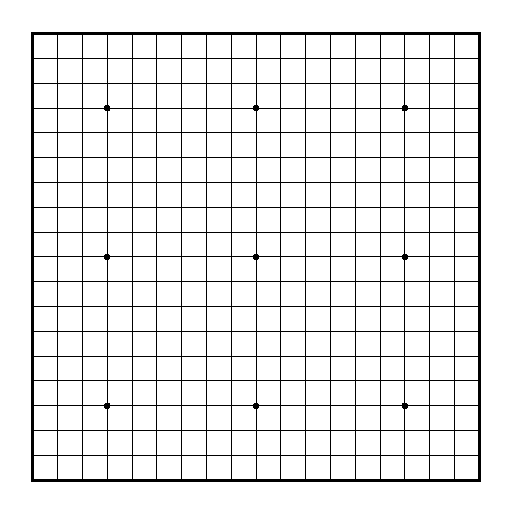
\includegraphics[width=.5\textwidth]{1 - Dia 1}
        \captionsetup{justification=centering}
        \caption*{\emph{Dia.\@~1}}
    \end{center}
    \vspace{-25pt}
\end{wrapfigure}

As pedras são colocadas em containeres chamados de potes. Há dois potes em um conjunto. Um pote é para as pedras pretas, e o outro, para as brancas.

A foto na capa mostra um exemplo de tabuleiro de Go com pernas em um ambiente tradicional japonês. O equipamento de Go pode ser obtido em uma grande gama de qualidade, desde conjuntos muito baratos àqueles custando dezenas de milhares de reais. É possível encontrar uma lista de equipamentos visitando o site da Kiseido: \href{https://www.kiseido.com}{\path{kiseido.com}}~\cite{kiseido}. Na verdade, você nem sequer precisa de um conjunto de Go para estudar ou jogar. É possível simplesmente baixar gratuitamente um programa chamado \emph{Go Write 2} que permite jogar e analisar posições (\href{https://www.gowrite.net/GOWrite2_download.html}{\path{gowrite.net/GOWrite2_download.html}})~\cite{gowrite}. Você também pode jogar partidas online sem custos com oponentes do mundo inteiro, através do servidor KGS (\href{https://www.gokgs.com}{\path{gokgs.com}})~\cite{kgs}. A força dos jogadores lá abrange desde iniciantes até profissionais.

O jogo de Go também pode ser jogado em pequenos tabuleiros, sem nenhuma mudança nas regras, e iniciantes são encorajados a jogar suas primeiras partidas em tabuleiros 9\(\times\)9. Já que uma partida 9\(\times\)9 pode ser finalizada em aproximadamente 10 minutos, esta é uma boa maneira de iniciantes se familiarizarem com as regras e as táticas básicas. Você talvez queira, a partir daí, então jogar algumas partidas em um tabuleiro $13\times13$ antes de progredir para o padrão oficial $19\times19$.
    \chapter{As Regras}\label{chap:regras}

\begin{itemize}
    \item[\textbf{Regra 1}] O tabuleiro começa vazio.
    \item[\textbf{Regra 2}] Preto sempre começa, e, a partir daí, Branco e Preto se alternam. 
    \item[\textbf{Regra 3}] Uma jogada consiste de colocar uma pedra de sua própria cor em uma intersecção vazia do tabuleiro, contanto que tal jogada seja legal, isto é, não conflite com as outras regras.
        
    Os \emph{Diagramas 1 a 3} demonstram uma abertura típica no tabuleiro 9x9. Uma vez jogadas, as pedras permanecem onde estão --- a não ser que capturadas, vide a \emph{Regra 5} ---; elas não podem ser fisicamente movidas para outros pontos. Exceto com pouquíssimas exceções causadas pela \emph{Regra 6}, uma jogada é irrestrita, isto é, você pode jogá-la onde quiser.
    \item[\textbf{Regra 4}] Um jogador pode passar o seu turno a qualquer momento.
    
    Passar geralmente ocorre em somente duas situações:
        
    \begin{enumerate}
        \item Perto do fim da partida;
        \item No início de um partida com pedras de compensação (\emph{handicap}).
    \end{enumerate}
    \item[\textbf{Regra 5}] Uma pedra ou um grupo de uma só cor conectado solidamente é capturado e removido do tabuleiro e mantido como prisioneiro quando todas as suas intersecções diretamente adjacentes são ocupadas pelo inimigo. Os 3 diagramas seguintes demonstram como capturas são executadas.
    \item[\textbf{Regra 6}] Um jogador não pode capturar suas próprias pedras. Ou seja, suicídio é ilegal.
\end{itemize}

\emph{Dia. 4.} Branco ocupa 3 de 4 pontos diretamente adjacentes à pedra preta; isto é, 3 de 4 liberdades. Diz-se que a pedra preta está em atari.

\emph{Dia. 5.} Branco 1 captura a pedra preta através da ocupação de sua última liberdade e a remove do tabuleiro.

\emph{Dia. 6.} Este é o resultado. As pedras capturadas são mantidas separadamente, tipicamente na tampa dos potes, que fica virada do avesso durante a partida.

\emph{Dia. 7 a 9} ilustram a captura na borda do tabuleiro.

\emph{Dia. 10 a 12} ilustram a captura  no canto do tabuleiro.

\emph{Dia. 13 a 15} demonstram  como um grupo de duas pedras solidamente conectado é capturado.

Um grupo solidamente conectado de 5 pedras é capturado nos \emph{Dia. 16 a 18}.

De acordo com a \emph{Regra 6}, é ilegal capturar suas próprias pedras. No \emph{Dia. 19}, as pedras brancas estão em atari. Não é possível salvá-las através da conexão em 1 no \emph{Dia. 20} pois se joga em sua própria liberdade, e as 3 pedras são deixadas sem nenhuma liberdade. Uma jogada assim é ilegal. Em outras palavras, ``a auto-captura é ilegal" ou ``o suicídio é ilegal". Entretanto, se for o turno preto, ele pode capturar as duas pedras brancas jogando em 1 no \emph{Dia. 21}.

A captura das pedras adversárias toma precedência sobre a auto-captura. No \emph{Dia 22}, as duas pedras pretas estão sob atari. Quando Branco 1 é jogado em \emph{Dia 23}, nem não há liberdades para tanto para 1 quanto para as duas pedras pretas à direita, mas são as pedras pretas, não as brancas, que são capturadas. O resultado é mostrado no \emph{Dia 24}. Se Preto quiser capturar, imediatamente, em \textbf{A}, ele pode mas não é obrigatório.

\section{30 Problemas de Captura e Resgate de Pedras}

Aqui estão 30 problemas. Depois de pensar sobre eles, você entenderá completamente como capturar pedras assim como, também, resgatar pedras em risco.

\section{Respostas aos Problemas de 1 a 30}

\begin{itemize}
  \item[\textbf{Resposta ao Problema 1}]
      Preto 1 no \emph{Dia. 1} captura um pedra.

      Se Preto joga 1 no \emph{Dia. 2}, Branco pode resgatar sua pedra através da extensão de 2.
  \item[\textbf{Resposta ao Problema 2}]
      Preto 1 no \emph{Dia. 1} captura uma pedra.

      Se Preto conecta em 1 no \emph{Dia. 2}, Branco pode resgatar sua pedra conectando em 2.
  \item[\textbf{Resposta ao Problema 3}]
      Preto 1 no \emph{Dia. 1} captura uma pedra.

      Se Preto conecta em 1 no \emph{Dia. 2}, Branco pode resgatar sua pedra conectando em 2.
  \item[\textbf{Resposta ao Problema 4}]
      Preto 1 no \emph{Dia. 1} captura duas pedras.

      Se Preto joga 1 no \emph{Dia. 2}, Branco pode resgatar suas pedras estendendo em 2.
  \item[\textbf{Resposta ao Problema 5}]
      Preto 1 no \emph{Dia. 1} captura duas pedras.

      Se Preto estende para 1 no \emph{Dia. 2}, Branco pode resgatar suas pedras conectando em 2.
  \item[\textbf{Resposta ao Problema 6}]
      Preto 1 no \emph{Dia. 1} captura as duas pedras marcadas.

      Se Preto estende para 1 no \emph{Dia. 2}, Branco pode resgatar suas duas pedras capturando as duas pedras pretas com 2.
  \item[\textbf{Resposta ao Problema 7}]
      Preto 1 no \emph{Dia. 1} captura duas pedras.

      Se Preto faz atari com 1 em \emph{Dia. 2}, Branco pode resgatar suas pedras e capturar duas do Preto com 2.
  \item[\textbf{Resposta ao Problema 8}]
      Preto 1 no \emph{Dia. 1} captura duas pedras.

      \emph{Dia. 2} mostra o resultado desta captura.
  \item[\textbf{Resposta ao Problema 9}]
      Preto 1 no \emph{Dia. 1} captura três pedras.

      Se Preto conecta em 1 no \emph{Dia. 2}, Branco pode resgatar sua pedra conectando em 2.
  \item[\textbf{Resposta ao Problema 10}]
      Preto 1 no \emph{Dia. 1} captura três pedras.

      Se Preto joga 1 no \emph{Dia. 2}, Branco pode resgatar as pedras em risco com a conexão em 2.
  \item[\textbf{Resposta ao Problema 11}]
      Preto 1 no \emph{Dia. 1} captura 3 pedras.

      Se Preto joga 1 no \emph{Dia. 2}, Branco pode salvar suas pedras e capturar as 4 pretas com 2.
  \item[\textbf{Resposta ao Problema 12}]
      Preto 1 em \emph{Dia. 1} captura uma pedra (crucial).

      Se Preto estende para 1 no \emph{Dia. 2}, Branco pode resgatar sua pedra conectando em 2.
  \item[\textbf{Resposta ao Problema 13}]
      Preto 1 no \emph{Dia. 1} captura cinco pedras.

      Se Preto joga 1 em \emph{Dia. 2} para escapar do atari, Branco pode resgatar suas cinco pedras conectando em 2.
  \item[\textbf{Resposta ao Problema 14}]
      Preto 1 no \emph{Dia. 1} captura cinco pedras.

      Se Preto conecta em 1 no \emph{Dia. 2}, Branco pode resgatar suas cinco pedras capturando quatro pedras com 2.
  \item[\textbf{Resposta ao Problema 15}]
      Preto pode resgatar sua pedra sob atari conectando em 1 no \emph{Dia. 1}.
      
      Se Preto faz atari com 1 no \emph{Dia. 2}, Branco pode capturar com 2.
  \item[\textbf{Resposta ao Problema 16}]
      Preto 1 no \emph{Dia. 1} resgata sua pedra em atari.

      Se Preto faz atari com 1 no \emph{Dia. 2}, Branco pode capturar uma pedra (crucial) com 2.
  \item[\textbf{Resposta ao Problema 17}]
      Preto 1 no \emph{Dia. 1} salva suas duas pedras sob atari.

      Se Preto faz atari com 1 no \emph{Dia. 2}, Branco pode capturar duas pedras com 2.
  \item[\textbf{Resposta ao Problema 18}]
      Preto 1 no \emph{Dia. 1} resgata sua pedra em atari.

      Se Preto faz atari com 1 no \emph{Dia. 2}, Branco pode capturar uma pedra com 2.
  \item[\textbf{Resposta ao Problema 19}]
      Preto 1 no \emph{Dia. 1} resgata suas três pedras em atari.

      Se Preto faz atari com 1 no \emph{Dia. 2}, Branco pode capturar três pedras com 2.
  \item[\textbf{Resposta ao Problema 21}]
      Preto 1 no \emph{1} resgata suas duas pedras em atari.

      Se Preto faz atari com 1 no \emph{Dia. 2}, Branco captura duas pedras com 2.
  \item[\textbf{Resposta ao Problema 22}]
      Branco não consegue escapar. Se ele rastejar na primeira linha com 1 a 10 no \emph{Dia. 1}, Preto captura oito pedras com 12.

      Após Branco 1 no \emph{Dia 2}, se Preto faz atari a partir da direita com 2, Branco pode escapar com 3 e 5.
  \item[\textbf{Resposta ao Problema 23}]
      Preto precisa fazer atari com 1 no \emph{Dia. 1}. Se Branco 2, Preto captura duas pedras com 3.

      Se Preto faz atari a partir da direita com 1 no \emph{Dia. 2}, ele possui somente uma liberdade, então Branco pode capturar três pedras com 2.
  \item[\textbf{Resposta ao Problema 24}]
      Preto precisa fazer atari com 1 no \emph{Dia. 1}. Se Branco 2, Preto faz atari novamente e suas pedras estão seguras. Se Branco \textbf{A}, Preto captura em \textbf{B}.

      Se Preto faz atari pelo topo com 1 em \emph{Dia. 2}, após Branco 2, as pedras marcadas ficam encarceradas.
  \item[\textbf{Resposta ao Problema 25}]
      Preto precisa fazer atari com 1 no \emph{Dia. 1}. Ele pode agora capturar três pedras com \textbf{A}. Se Branco \textbf{A}, suas pedras ainda estão sob atari.

      Se Preto faz atari com 1 no \emph{Dia. 2}, Branco conecta com 2 e suas pedras escapam.
  \item[\textbf{Resposta ao Problema 26}]
      Se Preto faz atari em 1 no \emph{Dia. 1}, ele captura quatro pedras. Se Branco joga 2, ele não possuirá nenhuma maneira de escapar depois de Preto 3.

      Se Preto faz atari com 1 no \emph{Dia. 2}, Branco estende com 2 e suas pedras escapam.
  \item[\textbf{Resposta ao Problema 27}]
      Preto deveria fazer atari com 1 no \emph{Dia. 1}. Preto pode agora capturar três pedras jogando em \textbf{A}. Se Branco \textbf{A}, suas pedras ainda estão em atari.

      Se Preto faz atari com 1 no \emph{Dia. 2}, Branco conecta com 2 e suas pedras escaparam.
  \item[\textbf{Resposta ao Problema 28}]
      As pedras pretas à direita estão em perigo, então ele precisa fazer atari na pedra marcada com 1 no \emph{Dia. 1}.

      Se Preto faz atari vindo debaixo com 1 no \emph{Dia. 2}, Branco faz atari com 2 e pode capturar em seguida com \textbf{A}.
  \item[\textbf{Resposta ao Problema 29}]
      Preto precisa fazer um duplo-atari  nas pedras marcadas com 1 no \emph{Dia. 1}. Ele pode agora capturar uma pedra em \textbf{A} ou \textbf{B}.

      Preto 1 em \emph{Dia 2} faz atari em somente uma pedra branca. Branco conecta com 2 e Preto não pode capturar nada.
  \item[\textbf{Resposta ao Problema 30}]
      Preto 1 no \emph{Dia. 1} é um duplo-atari, então Branco pode capturar uma das pedras marcadas em \textbf{A} ou \textbf{B}.
      
      Preto 1 no \emph{Dia. 2} faz atari em somente uma pedra. Branco conecta com 2 e Preto não pode capturar nada.
\end{itemize}
    \chapter{A Regra do Ko}

\begin{itemize}
  \item[\textbf{Regra 7}] Nenhuma posição de tabuleiro pode ser recriada.
\end{itemize}

Esta regra requer que todo movimente cria uma nova posição no tabuleiro. Sua principal função é prevenir ciclos infinitos de captura e recaptura em posições de ko como a exibida no \emph{Dia. 25}.

% TODO: Adicionar a origem do ko?

Na posição do \emph{Dia. 25}, suponha que seja o turno branco. Ele pode capturar uma pedra preta jogando em 1 no \emph{Dia. 26}. O resultado é mostrado no \emph{Dia. 27}.

Se Preto agora captura com 2 no \emph{Dia. 28}...

A posição do \emph{Dia. 29} é o resultado. Mas essa é a mesma posição do \emph{Dia. 25}. Pela \emph{Regra 7}, isso não é permitido, então Preto precisa jogar em outro lugar. Por exemplo, ele poderia jogar 2 no \emph{Dia. 30}. Isso oferece a Branco a oportunidade de conectar em 3, resolvendo o ko.

No \emph{Dia. 31}, é o turno Branco a jogar. Uma luta de ko está prestes a acontecer no entorno da pedra preta marcada, que está em atari.

Se Branco captura com 1 no \emph{Dia. 32}, Preto não pode imediatamente recapturar porque isso reverteria a posição de volta para o \emph{Dia. 31}, então ele jogará em outro lugar com Preto 2. Esse tipo de movimento é chamado de ameaça de ko.

Se Branco responde a essa ameaça com 3 no \emph{Dia. 33}, Preto pode recapturar com 4, pois a troca de Preto 2--Branco 3 faz com que a posição global do tabuleiro seja diferente do \emph{Dia. 31}. É agora a vez do Branco de encontrar uma ameaça de ko.

Branco corta com 5 no \emph{Dia. 34}. Preto poderia ignorar Branco 5 e capturar três pedras em \textbf{A}, e assim  resolver o ko, mas vamos supor qu eele responderia Branco 5 com 6. Branco pode agora recapturar o ko com 7. Preto precisa fazer outra ameaça de ko com 8. Talvez Branco ignorará essa ameaça e capturará quatro pedras com 9, finalizando a briga pelo ko. Preto obtém certa compensação com 10.
    \chapter{O Fim do Jogo}

\begin{itemize}
    \item[\textbf{Regra 8}] Duas passagens de turno consecutivas finalizam a partida. (Ou um dos jogadores pode desistir.)
    \item[\textbf{Regra 9}] No final da partida, toda pedra que não conseguir se salvar é removida do tabuleiro como prisioneira do adversário.
    \item[\textbf{Regra 10}] A pontuação de um jogador é o número de intersecções vazias que ele cercou menos o número de prisioneiros que ele perdeu para o adversário. A pontuação mais alta vence.
\end{itemize}

A partida no \emph{Dia.\@~35} está quase finalizada. Ambos Preto e Branco asseguraram seus respectivos territórios. Durante essa partida, Branco capturou diversos prisioneiros --- indicados pelas sete pedras pretas acima dos diagramas ---, e Preto capturou três pedras brancas.

\begin{figure}[h!]
    \centering
    \begin{subfigure}[t]{.3\textwidth}
        \centering
        
\includegraphics[width=.9\textwidth]{4 - Dia 35}
        \caption*{\emph{Dia.\@~35. Uma ameaça a de ko}}
    \end{subfigure}
    \hfill
    \begin{subfigure}[t]{.3\textwidth}
        \centering
        
\includegraphics[width=.9\textwidth]{4 - Dia 36}
        \caption*{\emph{Dia.\@~36. Branco captura}}
    \end{subfigure}
    \hfill
    \begin{subfigure}[t]{.3\textwidth}
        \centering
        
\includegraphics[width=.9\textwidth]{4 - Dia 37}
        \caption*{\emph{Dia.\@~37. Resolvendo o ko}}
    \end{subfigure}
    \caption*{\emph{Como capturas, Preto possui três pedras, e Branco, sete.}}
\end{figure}
  
Preto 1 no \emph{Dia.\@~36} não conquista nenhum ponto, mas ameaça a captura de uma pedra branca e o início de um ko, então Branco conecta com 2. Preto 3 e Branco 4 não ganham pontos também. Há pontos neutros que são jogados ao final da partida, somente para mais claramente delimitar os territórios. Não há mais pontos a serem disputados, então Preto 5 e Branco 6 são passagens de turno. De acordo com a \emph{Regra 8}, isso finaliza a partida.

A pedra branca marcada no \emph{Dia.\@~36} está morta: ela não consegue evitar de ser capturada. Portanto, de acordo com a \emph{Regra 9}, ela é removida do tabuleiro como prisioneira. O resultado dessa operação é visualizado no \emph{Dia.\@~37}. Note que Preto possui quatro prisioneiros brancos.

Vamos contar a pontuação.

\begin{figure}[h!]
    \centering
    \begin{subfigure}[t]{.3\textwidth}
        \centering
        
\includegraphics[width=.9\textwidth]{4 - Dia 38}
        \caption*{\emph{Dia.\@~38. O território preto}}
    \end{subfigure}
    \hfill
    \begin{subfigure}[t]{.3\textwidth}
        \centering
        
\includegraphics[width=.9\textwidth]{4 - Dia 39}
        \caption*{\emph{Dia.\@~39. O território branco}}
    \end{subfigure}
    \hfill
    \begin{subfigure}[t]{.3\textwidth}
        \centering
        
\includegraphics[width=.9\textwidth]{4 - Dia 40}
        \caption*{\emph{Dia.\@~40. O território é preenchido com prisioneiros}}
    \end{subfigure}
    \caption*{\emph{Como capturas, Preto possui três pedras, e Branco, sete.}}
\end{figure}

Preto cercou os pontos vazios marcados com \textbf{X} no \emph{Dia.\@~38}, e Branco cercou os pontos vazios marcados com \textbf{X} no \emph{Dia.\@~39}. Esses pontos vazios cercados são denominados de \emph{território}.

Para subtrair prisioneiros do território, os prisioneiros são colocados no tabuleiro dentro dos territórios pretos e brancos, como mostrado pelas pedras marcadas no \emph{Dia.\@~40}. Conte os territórios para cada lado e verá que Branco possui 6 pontos enquanto que Preto possui 5 pontos. Branco vence por um ponto.

Essas são as dez regras necessárias para se jogar Go. Há algumas poucas posições especiais e kos que são determinados por adjudicação. Essas posições são conhecidas como Precedentes da Nihon Kiin, mas elas ocorrem muito raramente em partidas.

As regras aqui apresentadas são as japonesas. Há outras também, a mais importante dentre essas outras sendo as regras chinesas. A maioria dos jogadores no ocidente utilizam as regras japonesas. Porém, se você for jogar Go na China, você terá de aprender sobre as regras chinesas. A principal diferença entre elas é o procedimento de contagem ao final da partida, mas, para basicamente todos os fins práticos, ambas são equivalentes. Isto é, elas não mudam a natureza do jogo. Para uma exposição dos diversos conjuntos de regras, assim como os Precedentes da Nihon Kiin, veja o livro \emph{The Go Player's Almanac}~\cite{bozulich_almanac}.
    \chapter{Partidas-Exemplo}\label{chap:cinco}

\section{Partida-Exemplo em um Tabuleiro \texorpdfstring{6$\times$6}{6x6}}

A partida a seguir ilustra jogadas perfeitas em um tabuleiro 6x6, o menor tamanho que Go é interessante de ser jogado.

\emph{Dia.\@~1} Isso pode ser chamado de abertura. Preto começa por tentar controlar o lado direito com 1 e 3, e Branco, controle do lado esquerdo com 2 e 4. Preto se dobra em volta de Branco com 5 e 7, e Branco resiste com 6 e 8.

\begin{figure}[h!]
  \centering
  \begin{subfigure}[t]{.3\textwidth}
      \centering
      
\includegraphics[width=.9\textwidth]{5 - Dia 1}
      \caption*{\emph{Dia.\@~1. (1-8)}}
  \end{subfigure}
  \hfill
  \begin{subfigure}[t]{.3\textwidth}
      \centering
      
\includegraphics[width=.9\textwidth]{5 - Dia 2}
      \caption*{\emph{Dia.\@~2. (9)}}
  \end{subfigure}
  \hfill
  \begin{subfigure}[t]{.3\textwidth}
      \centering
      
\includegraphics[width=.9\textwidth]{5 - Dia 3}
      \caption*{\emph{Dia.\@~3. (10-11)}}
  \end{subfigure}
\end{figure}

\emph{Dia.\@~2} Preto pressiona sua vantagem através do corte em 9. Isso põe as duas pedras marcadas em atari --- as pedras pretas estão ocupando todas as liberdades brancas exceto uma. Note que as pedras brancas marcadas não estão diretamente conectadas às outras pedras brancas.

\emph{Dia.\@~3} Branco resgata suas duas pedras pela conexão com 10, e a pedra preta marcada agora está em atari. Preto ignora isso e joga 11, colocando a pedra branca em atari.

\pagebreak

\emph{Dia.\@~4} Branco escapa do atari descendo para 12. Preto conecta com 13 para prevenir que Branco corte ali. A pedra preta marcada ainda está sob atari. Entretanto, ela não pode escapar, então Branco não se importa em capturá-la e corta em 14, colocando outra pedra preta em atari.

\begin{figure}[h!]
  \centering
  \begin{subfigure}[t]{.3\textwidth}
      \centering
      
\includegraphics[width=.9\textwidth]{5 - Dia 4}
      \caption*{\emph{Dia.\@~4. (12-14)}}
  \end{subfigure}
  \hfill
  \begin{subfigure}[t]{.3\textwidth}
      \centering
      
\includegraphics[width=.9\textwidth]{5 - Dia 5}
      \caption*{\emph{Dia.\@~5. (15-18)}}
  \end{subfigure}
  \hfill
  \begin{subfigure}[t]{.3\textwidth}
      \centering
      
\includegraphics[width=.9\textwidth]{5 - Dia 6}
      \caption*{\emph{Dia.\@~6. (19-21)}}
  \end{subfigure}
\end{figure}

\emph{Dia.\@~5} Preto joga um atari com 15 e Branco captura com 16, tomando um prisioneiro. Preto agora desce para 17, ameaçando jogar em 18 e desprivilegiar Branco de um ponto. Sendo assim, Branco precisa conectar em 18. Esse é o último movimento da partida e vale um ponto.

\emph{Dia.\@~6} Preto conecta com 19, preparando para tomar o último ponto neutro em 21. Branco não pode jogar em 21, então ele captura com 20, tomando outro prisioneiro.

\emph{Dia.\@~7} Após Preto 21 no \emph{Dia.\@~6}, não há mais pontos a serem ganhos ou disputados, então Branco passa. Preto também passa. De acordo com a \emph{Regra 8}, o jogo termina.

\begin{figure}[h!]
  \centering
  \begin{subfigure}[t]{.3\textwidth}
      \centering
      
\includegraphics[width=.9\textwidth]{5 - Dia 4}
      \caption*{\emph{Dia.\@~7. Partida finalizada}}
  \end{subfigure}
  \hspace{1cm}
  \begin{subfigure}[t]{.3\textwidth}
      \centering
      
\includegraphics[width=.9\textwidth]{5 - Dia 5}
      \caption*{\emph{Dia.\@~8}}
  \end{subfigure}
\end{figure}

\emph{Dia.\@~8} Branco possui dois prisioneiros, então ele os coloca no território preto --- as duas pedras marcadas. Os territórios são agora contados. Branco possui 6 pontos, e Preto, 9.

\textbf{Preto vence por 3 pontos.}

\pagebreak

\section{Perguntas e Respostas}

\begin{itemize}
    \item[\textbf{Pergunta}]
      Ao invés de 19 no \emph{Dia.\@~6}, será que Preto não poderia jogar atari em 2?
    \item[\textbf{Resposta}] 
      Se Preto fizer atari imediatamente com 1 em \emph{Dia.\@~9}, ele se colocaria em atari e perderia  duas pedras após a captura Branca com 2.

    \begin{figure}[h!]
      \centering
      \begin{subfigure}[t]{.3\textwidth}
          \centering
          
\includegraphics[width=.9\textwidth]{5 - Dia 9}
          \caption*{\emph{Dia.\@~9}}
      \end{subfigure}
      \hspace{1cm}
      \begin{subfigure}[t]{.3\textwidth}
          \centering
          
\includegraphics[width=.9\textwidth]{5 - Dia 10}
          \caption*{\emph{Dia.\@~10}}
      \end{subfigure}
    \end{figure}

    \item[\textbf{Pergunta}]
      Ao invés de capturar com 20 no \emph{Dia.\@~6}, será que Branco não poderia jogar no último ponto neutro em 21?
    \item[\textbf{Resposta}] 
      Se Branco jogar imediatamente em 1 no \emph{Dia.\@~10}, ele colocaria três de suas pedras em atari, e Preto procederia com a captura em 2.
    \item[\textbf{Pergunta}]
      Por que Branco passou no \emph{Dia.\@~7}? Por que ele não tenta invadir o território com 1 no \emph{Dia.\@~11}?
    \item[\textbf{Resposta}] 
      Não há regra que previna Branco de invadir. Mas ele percebe que seria de nenhuma utilidade. Preto responderia com 2 no \emph{Dia.\@~12}, colocando a pedra invasora em atari, e, quando Preto captura com 6, Branco perderia sua força invasora completamente.

    \begin{figure}[h!]
      \centering
      \begin{subfigure}[t]{.3\textwidth}
          \centering
          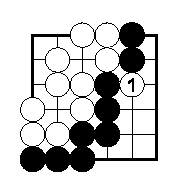
\includegraphics[width=.9\textwidth]{5 - Dia 11}
          \caption*{\emph{Dia.\@~11}}
      \end{subfigure}
      \hspace{1cm}
      \begin{subfigure}[t]{.3\textwidth}
          \centering
          
\includegraphics[width=.9\textwidth]{5 - Dia 12}
          \caption*{\emph{Dia.\@~12}}
      \end{subfigure}
    \end{figure}

    \item[\textbf{Pergunta}]
      Se Branco continuar insistindo na invasão, ele não conseguirá, no final, ocupar todos os pontos dentro do grupo Preto e, assim, capturá-lo?

    \begin{figure}[h!]
      \centering
      \begin{subfigure}[t]{.3\textwidth}
          \centering
          
\includegraphics[width=.9\textwidth]{5 - Dia 13}
          \caption*{\emph{Dia.\@~13}}
      \end{subfigure}
      \hfill
      \begin{subfigure}[t]{.3\textwidth}
          \centering
          
\includegraphics[width=.9\textwidth]{5 - Dia 14}
          \caption*{\emph{Dia.\@~14}}
      \end{subfigure}
      \hfill
      \begin{subfigure}[t]{.3\textwidth}
        \centering
        
\includegraphics[width=.9\textwidth]{5 - Dia 15}
        \caption*{\emph{Dia.\@~15}}
      \end{subfigure}
    \end{figure}

    \item[\textbf{Resposta}] 
      Ele é bem-vindo para tentar, como no \emph{Dia.\@~13}, mas ele não será bem sucedido. Após Branco 7 e 9, Preto esmaga aquelas duas pedras com 10 --- Branco não pode conectar no ponto 1-1, já que seria suicídio, um movimento ilegal. Branco põe o grupo preto de 11 pedras em atari com 11 no \emph{Dia.\@~14} e Preto captura duas pedras com 14. No final, Branco esgota os possíveis pontos de invasão. A posição agora aparenta ser \emph{Dia.\@~15} e Preto ainda vence por 3 pontos. Lembre-se que as pedras brancas voltarão para o território Branco quando a partida for contabilizada. Branco pode tentar novamente em \textbf{A}, mas Preto capturará imediatamente com \textbf{B}.
      
      O que faz com que o grupo preto inteiro no \emph{Dia.\@~15} seja invulnerável à captura são os vários buracos, ou olhos, que ele possui. Branco pode jogar somente uma pedra por vez, portanto ele jamais conseguirá preencher todos esses olhos simultaneamente, sem se suicidar, como ele deveria, para capturar o grupo preto.
    \item[\textbf{Pergunta}]
      Quantos olhos são necessários para que um grupo esteja seguro?
    \item[\textbf{Resposta}] 
      Ele precisa de dois, pelo menos. \emph{Dia.\@~16} mostra dois exemplos. Os dois grupos pretos estão vivos com dois olhos cada um. Na verdade, Branco não possui um movimento legal para atacar também. Branco, com seus dois grandes espaços de olhos, também está vivo. Preto pode jogar dentro do grupo branco, mas Branco pode facilmente capturar os invasores.

      \begin{figure}[h!]
        \centering
        \begin{subfigure}[t]{.3\textwidth}
            \centering
            
\includegraphics[width=.9\textwidth]{5 - Dia 16}
            \caption*{\emph{Dia.\@~16}}
        \end{subfigure}
        \hfill
        \begin{subfigure}[t]{.3\textwidth}
            \centering
            
\includegraphics[width=.9\textwidth]{5 - Dia 17}
            \caption*{\emph{Dia.\@~17}}
        \end{subfigure}
        \hfill
        \begin{subfigure}[t]{.3\textwidth}
          \centering
          
\includegraphics[width=.9\textwidth]{5 - Dia 18}
          \caption*{\emph{Dia.\@~18 Branco 3 em 1}}
        \end{subfigure}
      \end{figure}

      Você deveria também notar que os olhos precisam estar separados. O grupo preto no canto inferior esquerdo no \emph{Dia.\@~17} não está vivo, mas morto. Ele não consegue evitar de ser capturado. Talvez possa parecer que ele possui dois olhos, mas estes não separáveis ou distintos. Branco 1 no \emph{Dia.\@~18} coloca Preto em atari. Preto pode capturar com 2, mas Branco só joga novamente em 1 com 3, privando o grupo preto de sua última liberdade e, assim, capturando todas as cinco pedras pretas.

      Outra coisa sobre a qual se atentar é olho falso, como o que o grupo preto possui no canto superior direito do \emph{Dia.\@~18} em \textbf{A}. Esse grupo também está morto. Branco \textbf{A} captura as três pedras marcadas e põe as outras duas pedras sob atari.
    \item[\textbf{Pergunta}]
      Um grupo sempre precisa estar apto a criar dois olhos para estar vivo?

      \begin{figure}[h!]
        \centering
        \begin{subfigure}[t]{.3\textwidth}
            \centering
            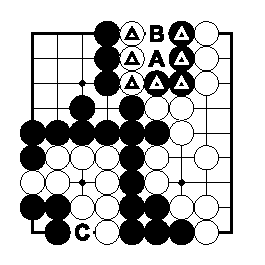
\includegraphics[width=.9\textwidth]{5 - Dia 19}
            \caption*{\emph{Dia.\@~19}}
        \end{subfigure}
      \end{figure}
    \item[\textbf{Resposta}] 
      Geralmente, mas há exceções. No \emph{Dia.\@~19}, o grupo preto marcado e o grupo branco não possuem nenhum olho, mas ambos compartilham liberdades. Nenhum dos lados pode atacar o outro jogando \textbf{A} ou \textbf{B} sem se colocar em atari, então nenhum dos lados deveria jogar nessa região, ou seja, ambos os grupos estão vivos. Este tipo de impasse local é chamado de \emph{seki}. Os pontos vazios entre as pedras marcadas não contam como território para nenhum dos lados.

      Há outro seki no canto inferior esquerdo do \emph{Dia.\@~19}. O grupo preto de três pedras e o grupo branco cercando-o ambos possuem um olho só e nenhum deles pode ocupar o ponto \textbf{C} entre eles sem se colocar sob atari. (O ponto \textbf{C} também não é território.)
\end{itemize}

\pagebreak

\section{Partida-Exemplo em um Tabuleiro \texorpdfstring{9$\times$9}{9x9}}

\emph{Dia.\@~1} A boa estratégia dita que movimentos de abertura sejam feitos na terceira linha ou acima, em relação às bordas do tabuleiro. Nesse caso, Preto 1 e Branco 2 são jogados nas quartas linhas.

\begin{figure}[h!]
  \centering
  \begin{subfigure}[t]{.3\textwidth}
      \centering
      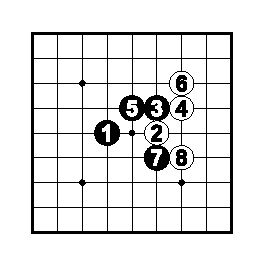
\includegraphics[width=.9\textwidth]{5 - Game 2 - Dia 1}
      \caption*{\emph{Dia.\@~1 (1-8)}}
  \end{subfigure}
  \hfill
  \begin{subfigure}[t]{.3\textwidth}
      \centering
      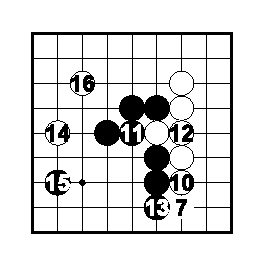
\includegraphics[width=.9\textwidth]{5 - Game 2 - Dia 2}
      \caption*{\emph{Dia.\@~2 (9-16)}}
  \end{subfigure}
  \hfill
  \begin{subfigure}[t]{.3\textwidth}
    \centering
    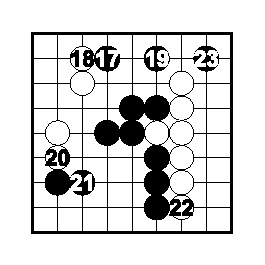
\includegraphics[width=.9\textwidth]{5 - Game 2 - Dia 3}
    \caption*{\emph{Dia.\@~3 (17-23)}}
  \end{subfigure}
\end{figure}

\emph{Dia.\@~2} Preto 11 faz atari na pedra branca, então Branco conecta em 12. Tendo construído um grupo vivo à direita, Branco invade o lado esquerdo com 14 e inicia a construção de outro grupo vivo à esquerda com 16.

\emph{Dia.\@~3} Branco defende seu grupo no lado esquerdo com 18 e 20, e, então, seu grupo à direita com 22. Preto pula para o lado direito com 23 e o fim de jogo se inicia. Pulos de um espaço como 19 e 23 são frequentemente boas jogadas.

\emph{Dia.\@~4} Branco detém a intrusão preta ao lado esquerdo com 24 e 26. As jogadas começam, a partir de agora, a focar nas bordas do tabuleiro.

\begin{figure}[h!]
  \centering
  \begin{subfigure}[t]{.3\textwidth}
      \centering
      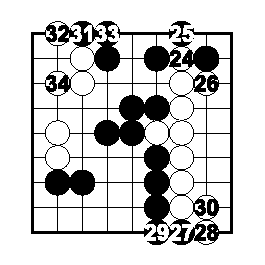
\includegraphics[width=.9\textwidth]{5 - Game 2 - Dia 4}
      \caption*{\emph{Dia.\@~4 (24-34)}}
  \end{subfigure}
  \hspace{1cm}
  \begin{subfigure}[t]{.3\textwidth}
      \centering
      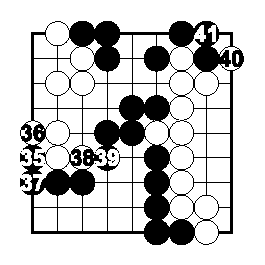
\includegraphics[width=.9\textwidth]{5 - Game 2 - Dia 5}
      \caption*{\emph{Dia.\@~5 (35-41)}}
  \end{subfigure}
\end{figure}

\emph{Dia.\@~5} O fim de jogo continua com Preto 35 até o atari de Branco 40.

\pagebreak

\emph{Dia.\@~6} Branco 50 é um sacrifício que, mais tarde, forçará Preto a conectar em 55. No final da partida, Branco perdeu um prisioneiro --- a pedra em 50 --- e Preto 53 é uma pedra morta.

\begin{figure}[h!]
  \centering
  \begin{subfigure}[t]{.3\textwidth}
      \centering
      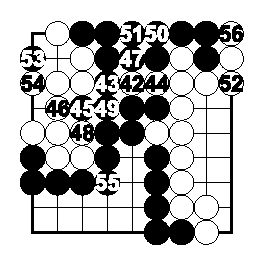
\includegraphics[width=.9\textwidth]{5 - Game 2 - Dia 6}
      \caption*{\emph{Dia.\@~6 (42-57)}}
  \end{subfigure}
  \hfill
  \begin{subfigure}[t]{.3\textwidth}
      \centering
      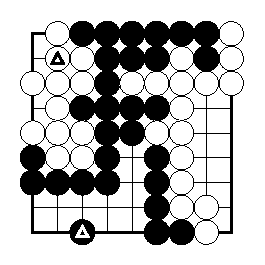
\includegraphics[width=.9\textwidth]{5 - Game 2 - Dia 7}
      \caption*{\emph{Dia.\@~2 Prisioneiros}}
  \end{subfigure}
  \hfill
  \begin{subfigure}[t]{.3\textwidth}
    \centering
    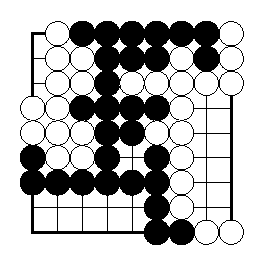
\includegraphics[width=.9\textwidth]{5 - Game 2 - Dia 8}
    \caption*{\emph{Dia.\@~8 Rearranjo}}
  \end{subfigure}
\end{figure}

\emph{Dia.\@~7} O prisioneiro branco é substituído dentro do território Branco, e a pedra preta morta --- 53 no \emph{Dia.\@~6} --- é removida e preenche o interior do território preto. Essas pedras são indicadas pelas pedras marcadas.

\emph{Dia.\@~8} É costumeiro rearranjar os territórios durante a contagem mais facilmente reconhecível em termos de múltiplos de 10. Nesta partida, Preto possui 11 pontos de território, e Branco, 13, portanto, Branco vence por dois pontos.
    \chapter{Estratégia de Abertura}

Para se tornar um jogador forte de Go, é necessário desenvolver duas habilidades:

\begin{enumerate}
    \item a habilidade de ler à frente movimento por movimento e prever os resultados de embates locais;
    \item a habilidade de intuir o que está acontecendo no tabuleiro como um todo.
\end{enumerate}

O balanço aproximadamente igualitário entre qualidades intuitivas e analíticas é grande parte da atratividade do Go. Na abertura, quando o tabuleiro consiste de majoritariamente espaço vazio, é intuição, e uma base de dados de conhecimento geral, que toma um papel dominante.

No tabuleiro 19x19, o tamanho oficial, é difícil de se assegurar território no início, então a partida usualmente começa com os jogadores espaçando suas pedras para formar grandes armações dentro das quais eles poderão brigar vantajosamente no futuro.

\emph{Dia. 1 a 3} mostra uma abertura típica no tabuleiro 19x19.

É geralmente muito mais fácil de se estabelecer bases nos cantos, como Preto e Branco o fazem com 1 a 4 no \emph{Dia. 1}. Uma ou duas pedras por canto é suficiente. Com 5, Preto estabelece um enclausuro de canto. Esse movimento delimita e vigia o território no canto. Não é ainda território seguro, uma vez que Branco possui múltiplas maneiras de invadi-lo. Mas Preto terá a vantagem em qualquer luta que se irromper ali. O tempo para a invasão branca será, assim, um fator crítico.

Aproximar-se do canto com Branco 6 no \emph{Dia. 2}, onde Preto possui somente uma pedra, é uma boa jogada. Isso frequentemente provoca lutas, como o curto conflito que se segue. Nos movimentos de 7 a 12, Preto assegura  o canto enquanto Branco constrói uma posição à direita. Essa sequência é um dos padrões-referência conhecidos como josekis.

Preto 13 no \emph{Dia. 13} é outro exemplo de outra aproximação. Branco 14 forma uma armação esparsa no canto inferior esquerdo do tabuleiro a partir da pedra branca marcada. A terceira ou a quarta linha é a melhor para extensões como esta. Preto desenvolve uma armação no topo com 15 e 17. Note Preto 17 na quarta linha, e Preto 15 e a pedra preta marcada na terceira linha. Isso constitui um balanço ideal de jogadas altas e baixas. As pedras na terceira linha defendem os flancos da posição preta enquanto que a pedra na quarta linha expande seu território para o centro.

\section{A Primeira Prioridade: Estabelecer uma Presença no Canto}

A abertura de uma partida de Go geralmente se inicia com ambos os lados estabelecendo presenças nos cantos. Os pontos a seguir são os cinco de referência que um jogador usualmente ocupa com seus primeiros movimentos.

\emph{Dia. 1. O ponto 3-3.} O intuito de Preto 1 no ponto 3-3 --- também conhecido como \emph{san-san} --- é assegurar o território no canto, apesar de que esse movimento não fornece muita influência no centro.

\emph{Dia. 2. O ponto-estrela.} Por ter jogado no ponto 4-4 --- também conhecido como ponto-estrela --- com 1, Preto almeja influência no centro.

\emph{Dia. 3. O ponto 3-4.} Quando Preto joga 1 no ponto 3-4 (\emph{komoku}), ele espera ganhar território ao longo do lado direito assim como algo no canto.

\emph{Dia. 4. O ponto 5-3.} Preto 1 no ponto 5-3 (\emph{mokuhazushi}) enfatiza o lado. Preto está disposto a conceder a maior parte do canto para Branco.

\emph{Dia. 5. O ponto 5-4.} Preto 1 no ponto 5-4 (\emph{takamoku}) concede o canto ao Branco. Ele almeja influência no centro e ao longo dos lados.

\section{Movimentos de Aproximação}


    \chapter{Táticas Elementares}

\section{Escadas}


    \chapter{Vida e Morte}

Nos \emph{Dias. 15 a 18} no \autoref{chap:cinco}, nós brevemente explicamos a diferença entre olhos reais e olhos falsos. Neste capítulo, mostraremos técnicas para a criação de olhos falsos nos grupos adversários, e explicaremos o conceito de olhos falsos.

\section{Olhos Falsos}

\emph{Dia.\@~1.} O grupo preto, que está confinado ao canto, possui somente um olho real, e um olho falso --- o ponto em \textbf{A} ---, portanto ele está morto. No final da partida, se Preto se recusar a aceitar que este grupo está morto, Branco pode demonstrá-lo através dos movimentos no \emph{Dia.\@~2}.

\begin{figure}[h!]
    \centering
    \begin{subfigure}[t]{.31\textwidth}
        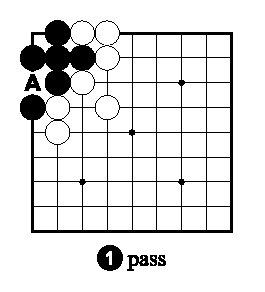
\includegraphics[width=1\textwidth]{8 - False Eyes - Dia 1}
        \caption*{\emph{Dia.\@~1}}
    \end{subfigure}
    \hspace{1cm}
    \begin{subfigure}[t]{.31\textwidth}
        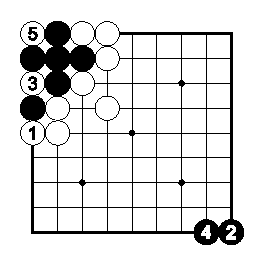
\includegraphics[width=1\textwidth]{8 - False Eyes - Dia 2}
        \caption*{\emph{Dia.\@~2. Preto 2 e 4 passam}}
    \end{subfigure}
\end{figure}

\emph{Dia.\@~2.} Teoricamente, no final da partida, Branco poderá capturar Preto com 1 a 5. Jogadores experientesnão jogariam tais movimentos, eles reconheceriam tal grupo como morto.

\pagebreak

\emph{Dia.\@~3.} Esse grupo preto não está morto ainda, mas Branco pode matá-lo.

\begin{figure}[h!]
    \centering
    \begin{subfigure}[t]{.31\textwidth}
        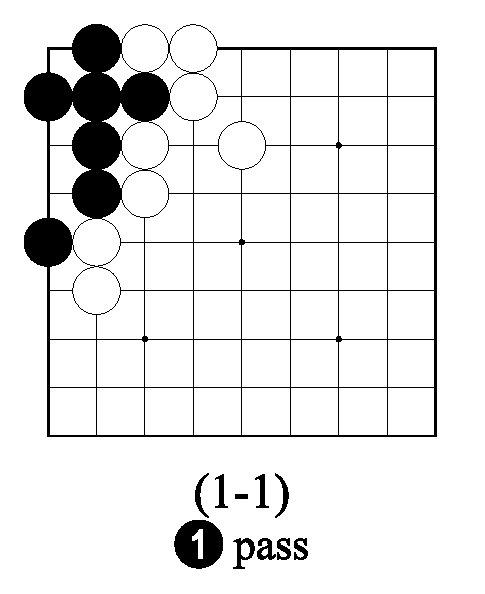
\includegraphics[width=1\textwidth]{8 - False Eyes - Dia 3}
        \caption*{\emph{Dia.\@~3}}
    \end{subfigure}
    \hfill
    \begin{subfigure}[t]{.31\textwidth}
        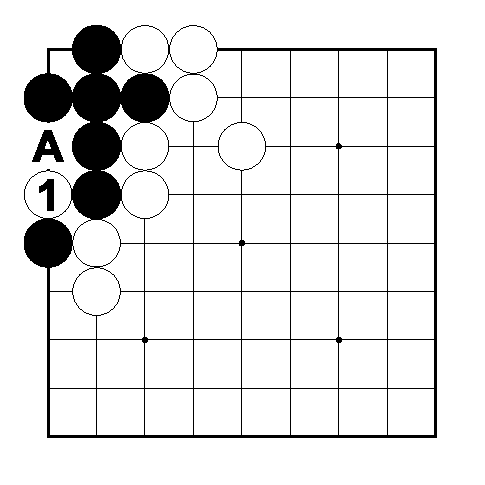
\includegraphics[width=1\textwidth]{8 - False Eyes - Dia 4}
        \caption*{\emph{Dia.\@~4}}
    \end{subfigure}
    \hfill
    \begin{subfigure}[t]{.31\textwidth}
        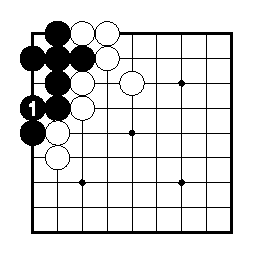
\includegraphics[width=1\textwidth]{8 - False Eyes - Dia 5}
        \caption*{\emph{Dia.\@~5}}
    \end{subfigure}
\end{figure}

\emph{Dia.\@~4.} Branco sacrifica uma pedra com 1, fazendo com que o segundo olho preto se torne falso. Se Preto capturar essa pedra com \textbf{A}, ele acabará com uma posição que é essencialmente idêntica ao \emph{Dia.\@~1}.

\emph{Dia.\@~5.} Para fazer dois olhos, Preto precisa conectar em 1. O grupo preto não poderá, então, mais ser morto.

\subsection{Exemplo 1}

O grupo preto no \emph{Dia.\@~1} está instável. Ele viverá ou morrerá, dependendo de qual será o próximo movimento.

\begin{figure}[h!]
    \centering
    \begin{subfigure}[t]{.31\textwidth}
        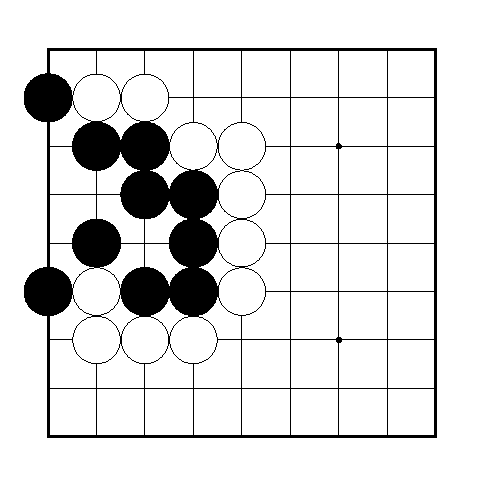
\includegraphics[width=1\textwidth]{8 - False Eyes - Example 1 - Dia 1}
        \caption*{\emph{Dia.\@~1. Instável}}
    \end{subfigure}
    \hspace{1cm}
    \begin{subfigure}[t]{.31\textwidth}
        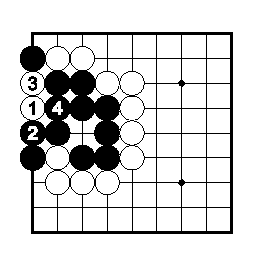
\includegraphics[width=1\textwidth]{8 - False Eyes - Example 1 - Dia 2}
        \caption*{\emph{Dia.\@~2. Morto}}
    \end{subfigure}
\end{figure}

Se Branco jogar primeiro, ele matará Preto com a colocação de 1 no \emph{Dia.\@~2}. Se Preto conectar com 2, Branco toma o ponto-chave de 3. Após a captura preta com 4\ldots

Branco sacrifica uma pedra com 5 no \emph{Dia.\@~3}, criando um olho falso naquele ponto. Preto não consegue mais fazer um segundo olho, portanto seu grupo está morto.

Se Preto jogar primeiro, ele poderá fazer um segundo olhopara seu grupo pela conexão de 1 no \emph{Dia.\@~4}. Se Branco \textbf{A}, Preto captura em \textbf{B} e obtém seus dois olhos.

\subsection{Exemplo 2}

O grupo preto no \emph{Dia.\@~1} está instável, incompleto. Ele viverá ou morrerá baseado no próximo movimento.

Se Branco jogar primeiro, ele poderá matar o grupo preto com o sacrifício de 1 no \emph{Dia.\@~2}. O ponto 1 agora é um olho falso. Capturar com 2 não ajuda Preto a criar um olho. Seu grupo está morto a partir daí.

O ponto \textbf{A} no \emph{Dia.\@~3} é um olho falso. Apesar de que Branco não precisa jogar lá, ele pode forçar Preto a jogar naquele ponto com o atari em \textbf{B}, se desafiado a demonstrar que o grupo Preto está morto.

Se Preto jogar primeiro, ele pode fazer um segundo olho para seu grupo conectando em 1 no \emph{Dia.\@~4}.

\subsection{Exemplo 3}

O grupo preto no \emph{Dia.\@~1} está incompleto. Vida ou morte dependem da próxima jogada.

Se Branco jogar primeiro, ele poderá jogar 1 no \emph{Dia 2} e transformar o olho em \textbf{A} em um olho falso. Preto está morto.

Se for turno preto, ele pode tornar o ponto \textbf{A} no \emph{Dia.\@~3} em um olho verdadeiro conectando em 1. 

\section{Espaço de Olho e Forma de Olho}

Quando um grupo cerca um espaço contíguo aberto de vários pontos, a questão de se esse espaço será suficientemente grande para assegurar dois olhos surge.

\emph{Dia.\@~1.} O grupo preto possui um espaço de três intersecções como olho, e seu status é instável.

\emph{Dia.\@~2.} Se Preto jogar 1, ele está vivo, pois possui dois olhos separados.

\emph{Dia.\@~3.} Porém, se Branco jogar 1, Preto está morto.

\emph{Dias. 4 e 5.} Os movimentos até Branco 11 nesses dois diagramas provam que o grupo Preto está morto. Branco simplesmente preenche todas as liberdades pretas mostradas. Preto não tem como se defender.

Aqui seguem mais alguns exemplos.

\emph{Dia.\@~6.} O grupo preto possui um olho de quatro espaços, e está vivo já.

\emph{Dia.\@~7.} Se Branco jogar em 1, Preto joga 2 e, novamente, ele está vivo com dois olhos separados.

\emph{Dia.\@~8.} Similarmente, se Branco jogar 1, Preto jogará 2 e, novamente, ele estará vivo com dois olhos separados.

\emph{Dia.\@~9.} Após Branco 1, Preto não pode passar ou ignorar o movimento branco. Branco continuará com 3 e Preto morrerá.

\emph{Dia.\@~10.} Branco pode demonstrar que Preto está morto jogando 5 a 9. Depois da captura por Preto em 10\ldots

\emph{Dia.\@~11.} Branco joga em 11, e a situação se torna clara: Preto não possui dois olhos.

\emph{Dia.\@~12.} O grupo preto está vivo ou morto, dependendo de quem for a vez.

\emph{Dia.\@~13.} Se for turno branco, e ele jogar em 1, o grupo preto está morto.

\emph{Dia.\@~14.} Se for turno preto, ele pode fazer três olhos jogando em 1.

\emph{Dia.\@~15.} O grupo preto é um quadrado de quatro espaços, e está morto já.

\emph{Dia.\@~16.} Mesmo se Preto jogar primeiro, tudo que ele pode fazer é jogar em 1 (ou qualquer outro ponto simétrico) e ameaçar fazer dois olhos jogando em 2. No entanto, Branco pode jogar 2 primeiro, e Preto é deixado sem uma resposta. Se ele jogar qualquer um entre \textbf{A} ou \textbf{B}, ele coloca todo seu grupo em atari.

\emph{Dia.\@~17.} Se Branco for desafiado a provar que o grupo Preto está morto, tudo que ele precisa fazer é jogar o atari em 4. Se Preto 5 capturar, Branco 6 joga novamente em 4, e todo o grupo preto inevitavelmente será capturado.

\emph{Dia.\@~18.} O grupo preto está vivo ou morto, dependendo de quem for o turno.

\emph{Dia.\@~19.} Se Branco jogar primeiro, ele pode matar Preto com 1. Esse movimento põe as cinco pedras pretas em atari. Se Preto conectar em \textbf{A}, todas as pedras estarão em atari. Após Branco 1, o grupo preto está morto, e a posição já está sedimentada.

\emph{Dia.\@~20.} Se for turno preto, ele pode viver jogando no ponto-chave de 1. Preto está vivo em seki. A posição fica como está. No final da partida, as três pedras brancas permanecerão no tabuleiro, e tanto Preto quanto Branco receberão zero pontos de território nesta região.

\emph{Dia.\@~21.} Se Branco resistir respondendo Preto 1, no \emph{Dia.\@~20}, com 2, Preto captura as quatro pedras brancas com 3.

\emph{Dia.\@~22.} Esse é o resultado da captura das pedras brancas no \emph{Dia.\@~21}. Preto está vivo com quatro pontos de território mais quatro pedras capturadas. Se Branco \textbf{A}, Preto ganha dois olhos jogando em \textbf{B}. Se Branco \textbf{B}, Preto \textbf{A}. Resistir, como no \emph{Dia.\@~21}, é uma perda de oito pontos para Branco.

\emph{Dia.\@~23.} O grupo preto possui um olho de cinco espaços. Ele está vivo ou morto, dependendo de quem for o turno.

\emph{dia. 24.} Depois de Branco 1, não mais nenhuma maneira com que Preto possa fazer dois olhos. Se necessário realmente capturar o grupo, Branco pode colocá-lo sob atari ocupando as intersecções marcadas com \textbf{X}. Se Preto, então, capturar com \textbf{A}, Preto acaba com um olho de quatro espaços, que é a mesma posição do \emph{Dia.\@~15}, onde mostramos que o grupo Preto está morto já.

\emph{Dia.\@~25.} Se for turno preto, ele poderá fazer dois olhos jogando no ponto-chave de 1.

O tópico de espaço de olho é minuciosamente contemplado no livro \emph{The Basics of Life and Death}~\cite{zeijst_bozulich_basics_of_life_and_death}, publicado pela Kiseido.

    \backmatter
    \bibliographystyle{plain}
    \bibliography{bibliografia}
\end{document}